\documentclass{article}
\usepackage{hyperref}
\usepackage{tabularx}
\usepackage{graphicx}
\usepackage{enumerate}
\usepackage{listings} 
\usepackage{float}

\begin{document}

\title{11-792 Project Report}
 
\author{Nicholas Gekakis, Boyue Li}
 
\maketitle
 
\section{Overview}

In this project, we are building a distributed question answering pipeline framework,
which allows users to easily configure multiple modules,
create complex pipelines and tune parameters automatically.

\section{Requirements}

    \subsection{Easy to configure and deploy}
    The framework should be easy to configure and deploy.

    \subsection{Save and resume}
    The framework should be save intermediate results so that it can be interrupted resume running at a later time.

    \subsection{Pipeline topology}
    The framework should be able to create pipelines with complex topologies.

    \subsection{Automatical parameter tuning}
    The framework should be able to automatically tune some parameters that have been exposed to the system by the pipeline developers.

    \subsection{Distributed parallel processing}
    The framework should support distributed parallel processing to handle large datasets and complicated pipelines (e.g. forked pipelines).

\section{Design}
    A pipeline is constructed from several independent modules.
    Users only need to specify
    \begin{enumerate}
        \item The correspondence between inputs and outputs
        \item The connections between modules
    \end{enumerate}
    The framework will automatically handle all execution.

    \subsection{Module}
    A module is the basic calculation unit which takes an arbitrary number of inputs and produces an arbitrary number of outputs.
    Every input and output is an information object defined below.
    A module also needs a description file to specify following fileds:
    \begin{itemize}
        \item Unique ID of the module.
        \item Name of the module.
        \item Number of inputs.
        \item Number of outputs.
        \item Data type of inputs.
        \item Data type of outputs.
        \item Number of parameters.
        \item Default values of parameters.
        \item Tuning interval of parameters.
        \item Tuning steps of parameters.
    \end{itemize}

    Figure \ref{fig:module_uml} is the UML diagram for the abstract
    \begin{figure}[H]
        \begin{center}
            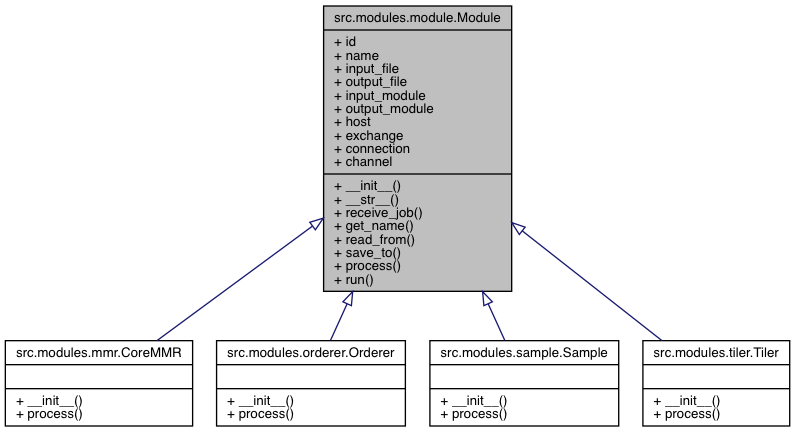
\includegraphics[width=0.3\textwidth]{fig/module_uml.png}
        \end{center}
        \label{fig:module_uml}
        \caption{UML diagram for abstract module class}
    \end{figure}


    \subsection{Information object}
    The information object used to pass data between modules contains the following fileds:

    \begin{itemize}
        \item Producing module: the module that produced this information object.
        \item Consuming module: the module that this information object to be passed to.
        \item Data path: the path to actual data file.
        \item Data type: the type of data (one of number, binary and string or user defined data type).
        \item Data size: the number of data instances.
    \end{itemize}

    \subsection{File format}
    A data file has a description file which contains the following fileds:

    \begin{itemize}
        \item The configuration applied to it.
        \item The timestamp when it is created.
        \item Data type.
        \item Data size.
    \end{itemize}

    Figure \ref{fig:infomation_obj_uml} is the UML diagram for the information object.

    \begin{figure}[H]
        \begin{center}
            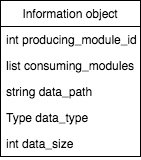
\includegraphics[width=0.3\textwidth]{fig/infomation_obj_uml.png}
        \end{center}
        \label{fig:infomation_obj_uml}
        \caption{UML diagram for information object}
    \end{figure}

    \subsection{Configuration file}
    We use YAML files to configure the framework.

    \subsection{Pipeline construction}
    We assign an unique ID to each module.
    Then we use these IDs to specify the connection of the pipeline.
    Therefore, we can easily design very complex pipelines.
    We use information object to pass data between modules.

    \begin{figure}[H]
        \begin{center}
            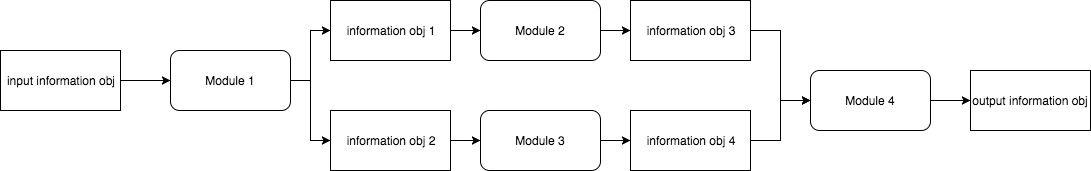
\includegraphics[width=1.2\textwidth]{fig/sample_pipeline.png}
        \end{center}
        \label{fig:sample_pipeline}
        \caption{A sample pipeline}
    \end{figure}
    Figure \ref{fig:sample_pipeline} shows a sample pipeline which passes the input information object
    through some modules and produces the output information object.


\section{Implementation}

\section{Experiments}
    \subsection{Dataset1}
    \subsection{Dataset2}
    \subsection{Dataset3}

\section{Conclusion}

\section*{Acknowledgements}

\end{document}



